\section{Evaluating on downstream tasks}
\label{sec:app}


\input{figures/corr_curve}


In this section, we apply our method to demonstrate its effectiveness on realistic downstream tasks. For evaluation, we exclude specific benchmarks that exhibit large performance variance (e.g., RTE) according to the performance traces reported in previous work~\citep{openelm2024} and our observations during pre-training.
Ultimately, we select the following benchmarks as our downstream tasks: Social IQA~\citep{sap2019socialiqa}, HellaSwag~\citep{zellers2019hellaswag}, PiQA~\citep{bisk2020piqa}, OpenBookQA~\citep{mihaylov2018can}, Lambada~\citep{paperno2016lambada}, SciQ~\citep{welbl2017crowdsourcing}, ARC Easy~\citep{clark2018think}, COPA~\citep{sarlin2020superglue}, RACE~\citep{lai2017race}, LogiQA~\citep{liu2020logiqa}, QQP~\citep{wang2018glue}, WinoGrande~\citep{sakaguchi2021winogrande}, and MultiRC~\citep{khashabi2018looking}. These benchmarks cover a diverse range of tasks, enabling a comprehensive evaluation of the real-world impact of \ourmethod. For each benchmark, we use normalized accuracy as the evaluation metric if provided by lm-eval-harness~\citep{eval-harness} else we use regular accuracy.


\subsection{Data mixture significantly impacts downstream performance}

\begin{table}[t]
    \centering
    \small
    \caption{We experiment with 64 models, each with 1B parameters trained on different data mixtures, and evaluate their performance across various benchmarks. The reported performance on each task is the average score from 0-shot to 5-shot settings, following~\citet{muennighoff2023scaling}. Here, we present the worst and best model performances on each task, and detailed experimental results for individual models can be found in Appendix~\ref{appendix:all_model_results}.}
    \vspace{1mm}
    \label{tab:worst_best_model_perf}
    \begin{tabular}{l|ccc}
    \toprule
     \textbf{Benchmark} & \textbf{Worst Model} & \textbf{Best Model} & $\Delta$ \\
     \midrule
        Social IQA~\citep{sap2019socialiqa} & 32.4 & 33.9 & 1.5 \\
        HellaSwag~\citep{zellers2019hellaswag} & 33.0 & 43.4 & 10.4 \\
        PiQA~\citep{bisk2020piqa} & 60.2 & 69.0 & 8.8 \\
        OpenBookQA~\citep{mihaylov2018can} & 25.8 & 31.2 & 5.4 \\
        Lambada~\citep{paperno2016lambada} & 18.9 & 33.5 & 14.6 \\
        SciQ~\citep{welbl2017crowdsourcing} & 76.7 & 82.9 & 6.2 \\
        ARC Easy~\citep{clark2018think} & 44.9 & 52.2 & 7.3 \\
        COPA~\citep{sarlin2020superglue}  & 61.5 & 70.5 & 9.0 \\
        RACE~\citep{lai2017race}  & 27.9 & 32.5 & 4.6 \\
        LogiQA~\citep{liu2020logiqa}  & 23.2 & 27.7 & 4.5 \\
        QQP~\citep{wang2018glue}  & 48.0 & 59.7 & 11.7 \\
        WinoGrande~\citep{sakaguchi2021winogrande} & 50.3 & 53.2 & 2.9 \\
        MultiRC~\citep{khashabi2018looking} & 47.6 & 55.7 & 8.1 \\
        \midrule
        Average Performance & 43.7 & 47.9 & 4.2 \\
    \bottomrule
    \end{tabular}
\end{table}

Initially, we train 64 models, each with 1B parameters, using different data mixtures.
Every model is trained on 25B tokens\footnote{We set the token quantity such that it is compute-optimal according to Chinchilla~\citep{hoffmann2022training}.} from the Pile dataset~\citep{the_pile_corpus}, with tokens allocated based on their corresponding domain weights.
Table~\ref{tab:worst_best_model_perf} presents the performance of the worst and best models on each downstream task. The reported performance is the average from 0-shot to 5-shot evaluations, scored using the lm-eval-harness evaluation framework~\citep{eval-harness,biderman2024lessons}. We find that the data mixture significantly impacts downstream performances, with the largest performance $\Delta$ reaching $14.6$ on the Lambada task. This underscores the importance of studying the optimal data mixture.

\subsection{Web corpora benefits downstream performance the most}

\begin{figure}[t]
    \centering
    \subfigure[Correlation between validation loss by domains of the Pile and downstream performance.]{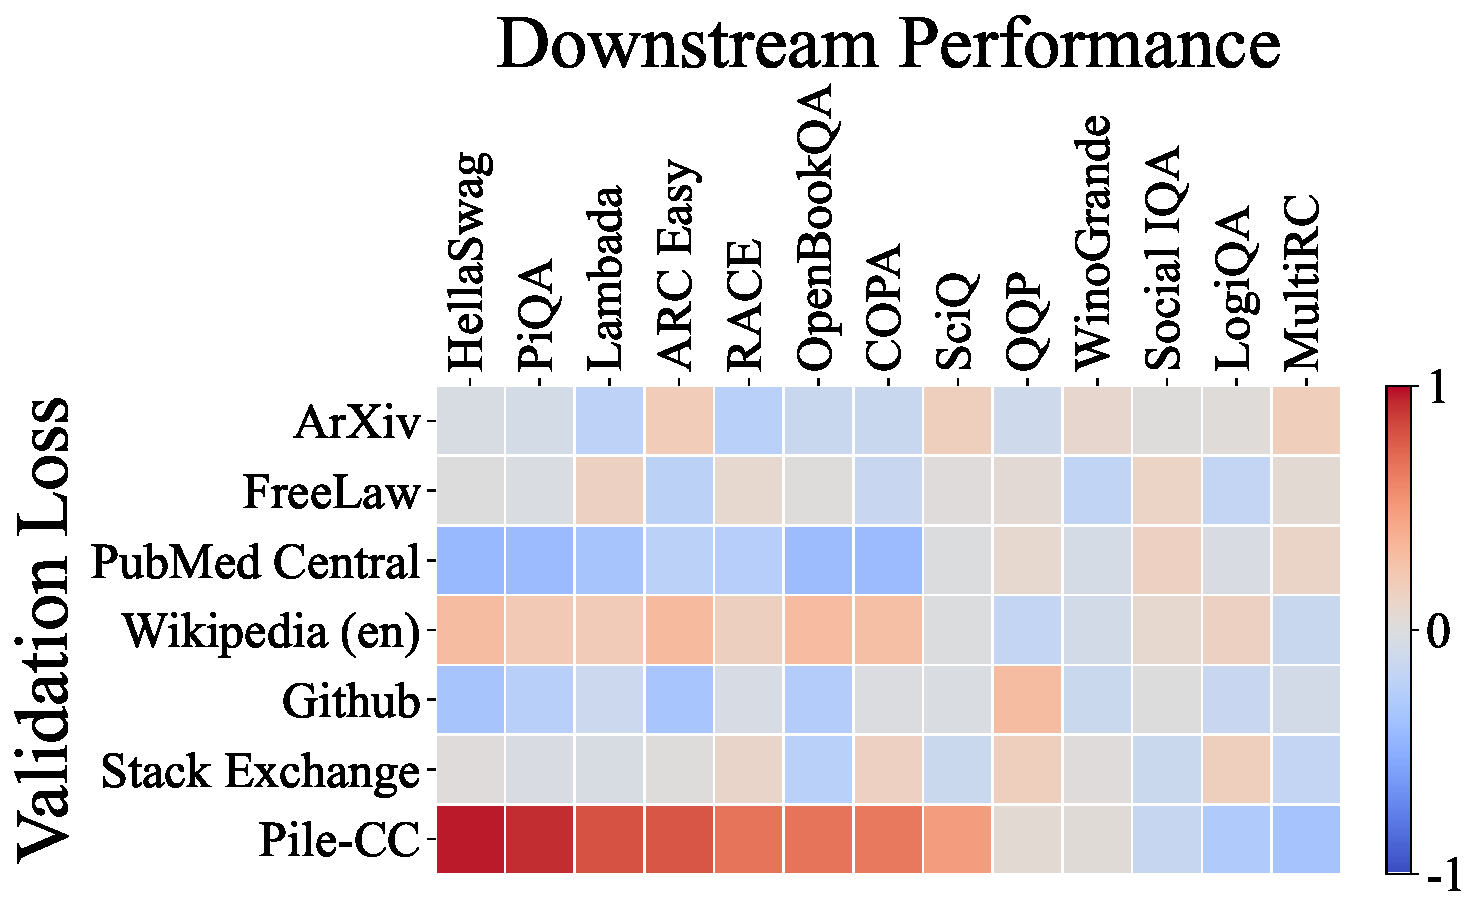
\includegraphics[height=0.28\textwidth]{figures/Domain_and_Task.pdf}}
    \hspace{1mm}
    \subfigure[Correlation between validation loss by URL domain within the Pile-CC subset and downstream performance.]
    {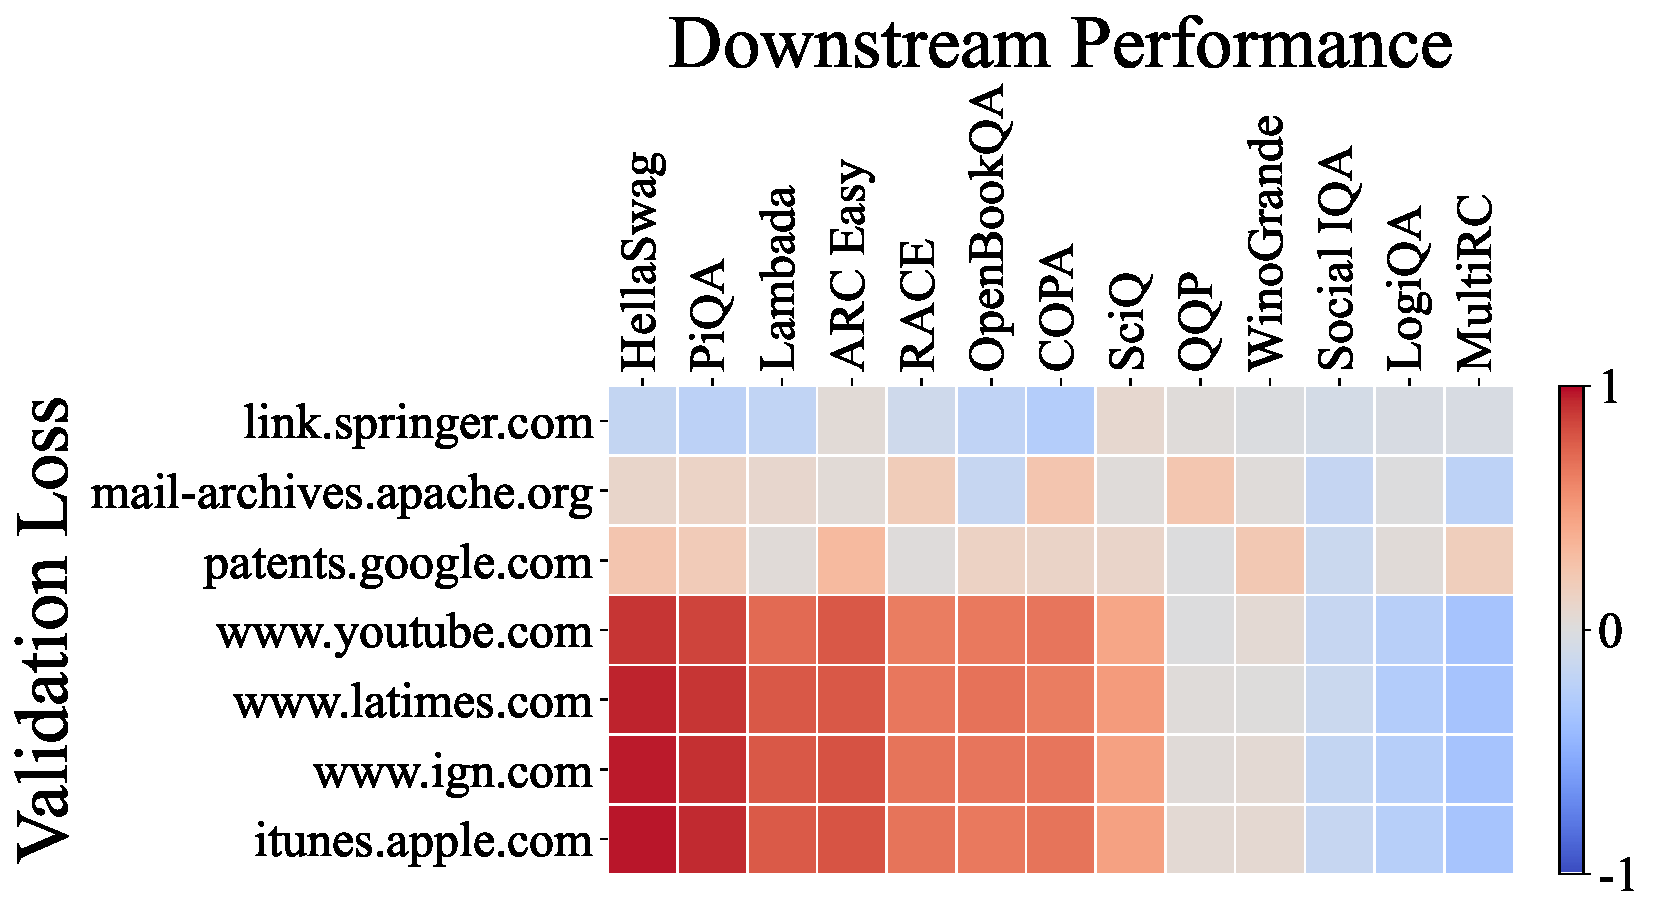
\includegraphics[height=0.28\textwidth]{figures/Domain_and_Task_c4100.pdf}}
    \caption{The correlation between validation losses across domains and downstream performance for the $64 \times$ 1B models. Note that we take the negative of the loss value when calculating the correlation, as this makes the visualization more intuitive. The same applies for Figure~\ref{fig:domain_interaction}. }
    \label{fig:domain-and-task}
\end{figure}

Next, we visualize the correlation between the validation losses of our 64 1B models across different domains and their performance on various downstream tasks in Figure~\ref{fig:domain-and-task} (a). Prior to visualization, we hypothesized that the validation loss on the Wikipedia (en) subset would exhibit a strong correlation with most downstream tasks, as it is a high-quality dataset, and many downstream tasks are derived from Wikipedia text. Similarly, previous work often takes WikiText~\citep{merity2016pointer} as a standard benchmark to indicate language model performance.

However, surprisingly, the validation loss on the Pile-CC dataset shows the strongest correlation with most downstream tasks. For instance, the correlation coefficient between the HellaSwag task and the Pile-CC validation loss is remarkably close to $1.0$.
This unexpected result challenges the conventional assumption that WikiText is the most representative dataset for evaluating LLMs.
Furthermore, this result aligns with the findings of previous studies~\citep{gadre2024language, huang2024compression}, which discovered that the validation loss on the web dataset closely relates to downstream performance. 

Moreover, we analyze the correlation between the loss of models on the C4100Domain validation set~\citep{paloma2023allen}, which is taken from the C4 dataset~\citep{2019t5} and supposed to share a similar distribution as Pile-CC since they are all derived from the CommonCrawl corpus. Since CommonCrawl is a collection of diverse domains, we would expect the correlation between the loss of each domain and the downstream tasks to vary. However, surprisingly more than 85\% of the domains exhibit a very strong correlation with Pile-CC (full correlation graph in Appendix~\ref{appendix:correaltion_graph}).
This is exemplified by the \texttt{www.ign.com} domain, which closely mirrors the overall correlation graph of Pile-CC, as illustrated in Figure~\ref{fig:domain-and-task} (b).
It also suggests that the high correlation between Pile-CC and downstream task performance may be attributed to its \textit{diverse coverage across various topics and domains}.\looseness=-1

\subsection{Data mixture by \ourmethod improves downstream performance}
\label{sec:no_pile_exper}


\begin{table}[tb]
    \centering
    \small
    \caption{Performance comparison of different data selection methods. Human refers to the weights put forth in The Pile~\citep{the_pile_corpus}, Pile-CC to only training on the Pile-CC component, PPL to using the perplexity filtering methods from \citet{zachary2024perplexed}, ODM to the weights from \citet{albalak2023efficient} and DoReMi to the weights from \citet{xie2023doremi}. The reported performance on each task is the average score from 0-shot to 5-shot settings, while the highest score on each task is highlighted in bold. We estimate the compute (measured in FLOPs) required to arrive at the training data mixture.\looseness=-1}
    \label{tab:downstream_perf_our}
    \vspace{1mm}
    \begin{tabular}{l|cccccc}
    \toprule
         \textbf{Benchmark} & \textbf{Human} & \textbf{DoReMi} & \textbf{PPL} & \textbf{ODM} & \textbf{Pile-CC} & \textbf{\ourmethod} \\
    \midrule
        Social IQA~\citep{sap2019socialiqa} & 33.6 & 33.4 & 33.3 & 33.7 & 33.2 & \textbf{33.8}  \\ 
        HellaSwag~\citep{zellers2019hellaswag} & 37.4 & 43.4 & 43.1 & 37.2 & 44.1 & \textbf{44.2}  \\ 
        PiQA~\citep{bisk2020piqa} & 65.0 & 68.3 & 68.5 & 64.4 & 69.2 & \textbf{69.3}  \\ 
        OpenBookQA~\citep{mihaylov2018can} & 28.2 & 30.3 & 30.3 & 30.0 & \textbf{31.1} & 30.3  \\ 
        Lambada~\citep{paperno2016lambada} & 29.8 & 32.1 & \textbf{35.4} & 29.6 & 33.2 & {34.2}  \\
        SciQ~\citep{welbl2017crowdsourcing} & 80.1 & 81.6 & 78.6 & 79.8 & 81.8 & \textbf{82.8}  \\ 
        ARC Easy~\citep{clark2018think} & 49.4 & 50.6 & 50.5 & 47.9 & \textbf{51.8} & 51.7  \\ 
        ARC Challenge~\citep{clark2018think} & 26.3 & 26.1 & 25.9 & 25.6 & \textbf{26.7} & 25.7  \\ 
        COPA~\citep{sarlin2020superglue} & 66.7 & 68.5 & 69.2 & 68.2 & 65.8 & \textbf{70.2}  \\ 
        RACE~\citep{lai2017race} & 29.0 & 31.3 & 31.5 & 29.7 & \textbf{31.8} & 31.3 \\ 
        LogiQA~\citep{liu2020logiqa} & 25.5 & {26.4} &  27.5 & 25.6 & \textbf{27.6} & 25.8  \\ 
        QQP~\citep{wang2018glue} & 52.4 & 56.6 & 50.0 & 53.1 & 57.0 & \textbf{58.3}  \\ 
        WinoGrande~\citep{sakaguchi2021winogrande} & \textbf{53.1} & 52.2 & 52.8 & 51.8 & 52.1 & \textbf{53.1}  \\ 
        MultiRC~\citep{khashabi2018looking} & \textbf{54.3} & 53.8 & 50.4 & 53.3 & 50.3 & 51.7 \\
        \midrule
        Estimated FLOPs & 0 & $3.7\text{e}19$ & $1.8\text{e}19$ & 0 & 0 & $3.5\text{e}18$ \\
        Average Performance & 45.1 & 46.8 & 46.2 & 45.0 & 46.8 & \textbf{47.3} \\
        Best On & 2 / 14 & 0 / 14 & 1 / 14 & 0 / 14 & 5 / 14 & \textbf{7 / 14} \\
    \bottomrule
    \end{tabular}
\end{table}

Previous work has shown that the data mixture method can accelerate LLM pre-training by achieving a smaller validation loss (or perplexity) using less training tokens~\citep{xie2023doremi}. However, a critical challenge is determining \textit{which validation loss to optimize}.
While the intuitive approach is to minimize loss across all domains, our analysis of 1M training logs reveals significant practical challenges.
Therefore, instead of pursuing a broad optimization strategy, we strategically focus on minimizing validation loss on Pile-CC, which allows for meaningful progress by leveraging Pile-CC which most consistently predicts overall model performance on downstream tasks.

We implement two approaches to determine the data mixture.
The first approach relies on human intuition.
Since Pile-CC and its own distribution should be the closest match, we hypothesized that pre-training solely on Pile-CC might yield better performance than baselines.
The second approach leverages \ourmethod, using the Pile-CC validation loss as the target variable. We employed LightGBM to predict the data mixture which can minimize the Pile-CC validation loss. \looseness=-1

We evaluate our proposed approaches against robust benchmarks, including human-curated selections for the Pile corpus~\citep{the_pile_corpus}, a sample-level perplexity-based filtering method (PPL)~\citep{zachary2024perplexed}, an online group-level method Online Data Mixing (ODM)~\citep{albalak2023efficient}, and the flagship group-level method DoReMi~\citep{xie2023doremi}. 
For ODM and DoReMi, we obtain the data mixture directly from their reported best domain weights and re-normalize it across the available 17 domains. This may result in sub-optimal performance for them compared to the originally reported results. As shown in Table~\ref{tab:downstream_perf_our}, both Pile-CC Only and \ourmethod demonstrate strong performance compared to the baselines. On the widely used HellaSwag benchmark, \ourmethod shows an improvement of $6.8$ over Human selection. Additionally, \ourmethod beats all other three methods on the task performance in 7 out of 14 cases and yields the highest average score. The surprisingly strong performance of Pile-CC Only reinforces the conclusion from our previous section: web corpora benefits on downstream performance. Finally, \ourmethod surpasses the Best Model in Table~\ref{tab:worst_best_model_perf}, demonstrating that our automatic data mixture approach is more efficient than random search.


\begin{figure}[!t]
\centering
\small
\begin{tikzpicture}
\begin{axis}[
at={(0em,0)},
width=.4\textwidth, height=.3\textwidth ,
xtick={1,5,...,25},
ytick={2.75, 3.0, ..., 4.5},
grid style=dashed,
ylabel={Validation\ \ Loss},
xlabel={{Training Tokens (B)}},
xlabel style={align=center,yshift=0em},
ylabel style={yshift=0},
y tick style={opacity=0},
ymajorgrids=true,
xmajorgrids=true,
tick align=inside,
legend pos=outer north east,
yticklabel style={/pgf/number format/precision=2,/pgf/number format/fixed zerofill},
legend style={yshift=-0.5em,xshift=-9.7em,legend cell align=left,legend plot pos=right,draw=none},
xmin=-1,
xmax=26,
ymin=2.7,
ymax=4.0]
    \addplot[
        red!60,mark=pentagon*,mark size=1.2pt,thick,mark options={fill=white,draw=red,line width=0.5pt}
        ]
        coordinates {
(1, 3.820050001)
(3, 3.443202972)
(5, 3.316340208)
(7, 3.238892794)
(9, 3.184519053)
(11, 3.141363859)
(13, 3.104880571)
(15, 3.072213173)
(17, 3.04462266)
(19, 3.021899939)
(21, 3.00503087)
(23, 2.994301796)
(25, 2.989006996)
        };
      \addplot[
        blue!60,mark=square*,mark size=1.2pt,thick,mark options={fill=white,draw=blue,line width=0.5pt}
        ]
        coordinates {
(1, 3.564236641)
(3, 3.212352514)
(5, 3.092962027)
(7, 3.025346518)
(9, 2.975091696)
(11, 2.93320632)
(13, 2.89994359)
(15, 2.869195461)
(17, 2.844691038)
(19, 2.824284554)
(21, 2.808733463)
(23, 2.798743486)
(25, 2.793961763)
        };
      \addplot[
        orange!60,mark=triangle*,mark size=1.2pt,thick,mark options={fill=white,draw=orange,line width=0.5pt}
        ]
        coordinates {
(1, 3.575109243)
(3, 3.201750994)
(5, 3.07610321)
(7, 3.006507158)
(9, 2.955598593)
(11, 2.911984682)
(13, 2.876117468)
(15, 2.846674204)
(17, 2.820066452)
(19, 2.798643112)
(21, 2.782349825)
(23, 2.771711111)
(25, 2.76705265)
        };
\end{axis}
\begin{axis}[
at={(20em,0)},
width=.4\textwidth, height=.3\textwidth ,
xtick={1,5,...,25},
ytick={2.75, 3.0, ..., 4.5},
grid style=dashed,
ylabel={Validation\ \ Loss},
xlabel={{Training Tokens (B)}},
xlabel style={align=center,yshift=0em},
ylabel style={yshift=0},
y tick style={opacity=0},
ymajorgrids=true,
xmajorgrids=true,
tick align=inside,
legend pos=outer north east,
yticklabel style={/pgf/number format/precision=2,/pgf/number format/fixed zerofill},
legend style={yshift=-2em,xshift=0.5em,legend cell align=left,legend plot pos=right,draw=none},
xmin=-1,
xmax=26,
ymin=3.0,
ymax=4.50]
    \addplot[
        red!60,mark=pentagon*,mark size=1.2pt,thick,mark options={fill=white,draw=red,line width=0.5pt}
        ]
        coordinates {
(1, 4.305472374)
(3, 3.702566862)
(5, 3.542406321)
(7, 3.463979483)
(9, 3.402868032)
(11, 3.355190039)
(13, 3.315196753)
(15, 3.28206563)
(17, 3.254812002)
(19, 3.230043173)
(21, 3.213106632)
(23, 3.201158285)
(25, 3.196551085)
        };
      \addplot[
        blue!60,mark=square*,mark size=1.2pt,thick,mark options={fill=white,draw=blue,line width=0.5pt}
        ]
        coordinates {
(1, 4.17596674)
(3, 3.586002111)
(5, 3.438609838)
(7, 3.364253044)
(9, 3.311367512)
(11, 3.271058083)
(13, 3.238744497)
(15, 3.212095261)
(17, 3.186464071)
(19, 3.167378426)
(21, 3.153804779)
(23, 3.14490509)
(25, 3.140860558)
        };
      \addplot[
        orange!60,mark=triangle*,mark size=1.2pt,thick,mark options={fill=white,draw=orange,line width=0.5pt}
        ]
        coordinates {
(1, 4.119034767)
(3, 3.535004854)
(5, 3.393175602)
(7, 3.316093445)
(9, 3.265641689)
(11, 3.225485563)
(13, 3.195032358)
(15, 3.166511536)
(17, 3.141429901)
(19, 3.121953964)
(21, 3.107906342)
(23, 3.099808216)
(25, 3.095982313)
        };
        \legend{{Human},{DoReMi},{\ourmethod}}
\end{axis}
\end{tikzpicture}
\vspace{-4mm}
\caption{\textbf{Left}: The validation loss on Pile-CC of different methods with Pile-CC in the pre-training corpus. \textbf{Right}: The validation loss on Pile-CC excluding Pile-CC in the pre-training.}
\label{fig:loss_curve}
\vspace{-1mm}
\end{figure}



While the Pile-CC validation loss is an informative indicator for downstream performance, it may not generalize to every task of interest. Sometimes we may not be able to assume that the validation set stems from a similar data distribution as the training set, but rather face an out-of-distribution scenario.
To verify the effectiveness of our method in out-of-distribution scenarios, we fully exclude the Pile-CC domain from the pre-training corpus and use the remaining domains to find the optimal data mixture that minimizes Pile-CC validation loss. As illustrated in Figure~\ref{fig:loss_curve} (right), our proposed method still outperforms baseline approaches. This demonstrates that \ourmethod is robust regardless of whether the target domain is in- or out-of-distribution.
We additionally provide the results of regression evaluation under this setting in Figure~\ref{tab:linear_vs_lightgbm_1M_OOD}.

\subsection{Domain interactions are challenging for humans to understand}\label{sec:domain_interaction}


\begin{figure}[t]
    \centering
    \subfigure{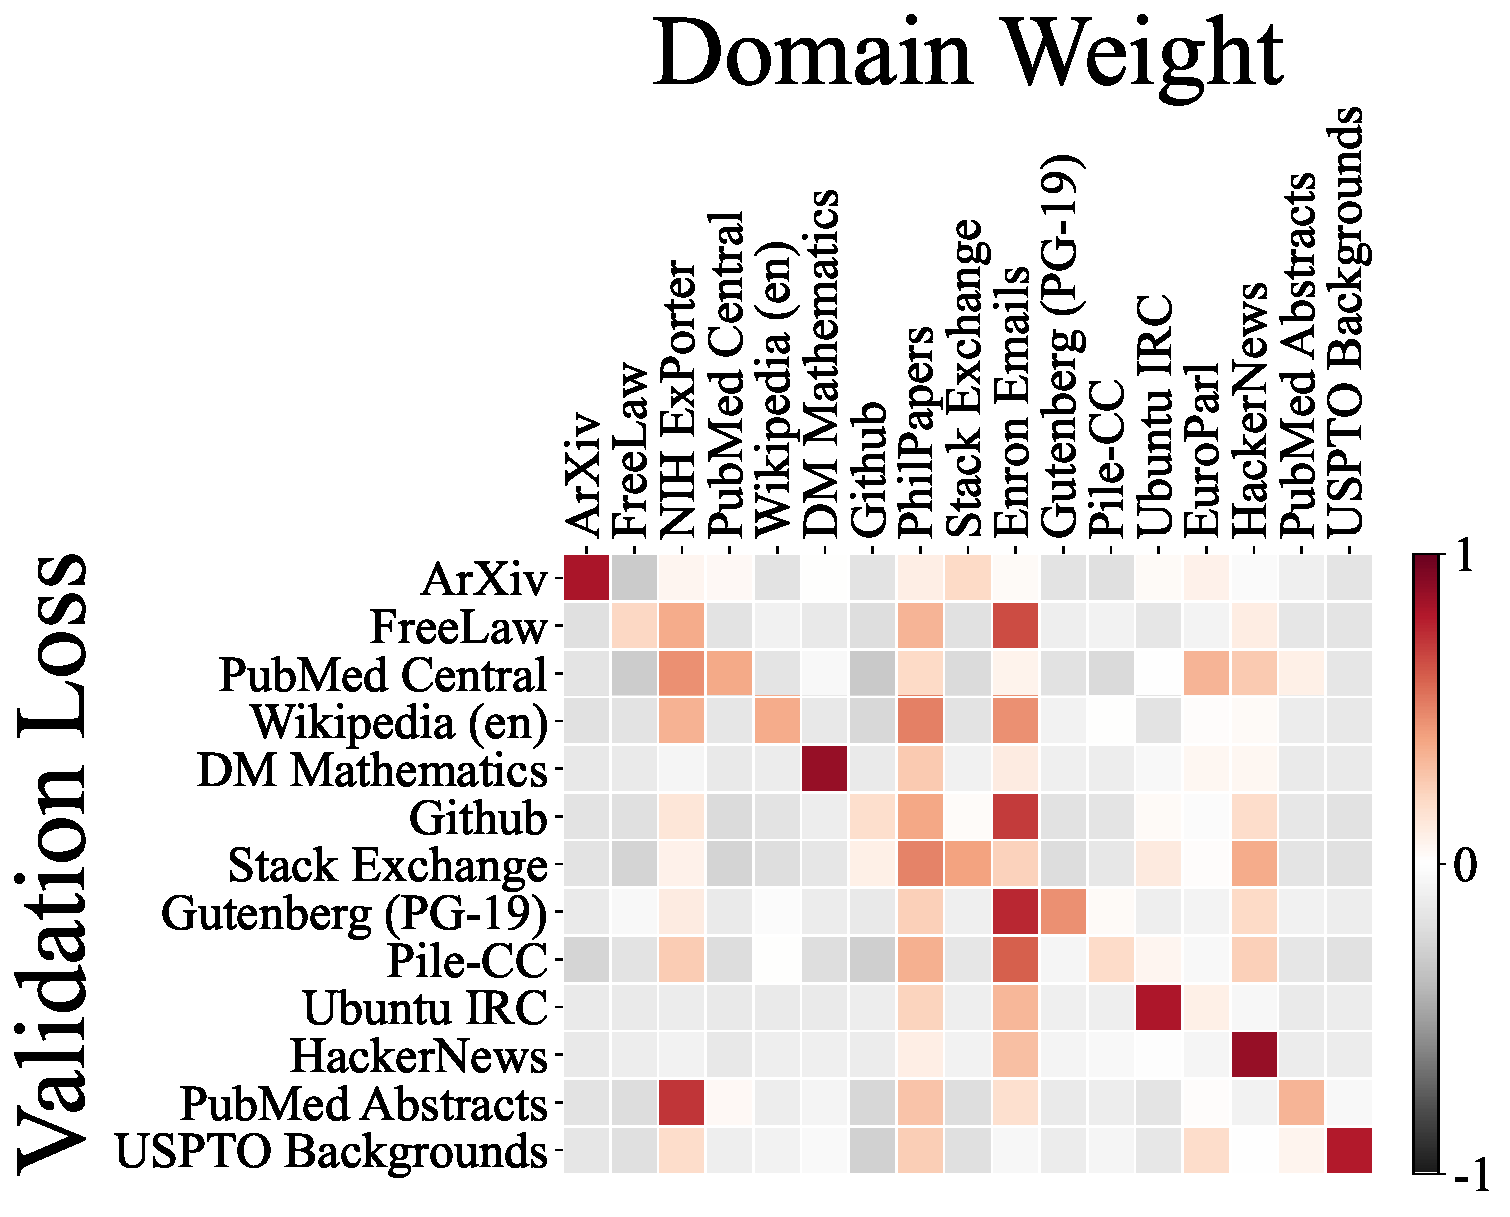
\includegraphics[height=.285\textwidth]{figures/1M_pile_4B_w.pdf}}
    \subfigure{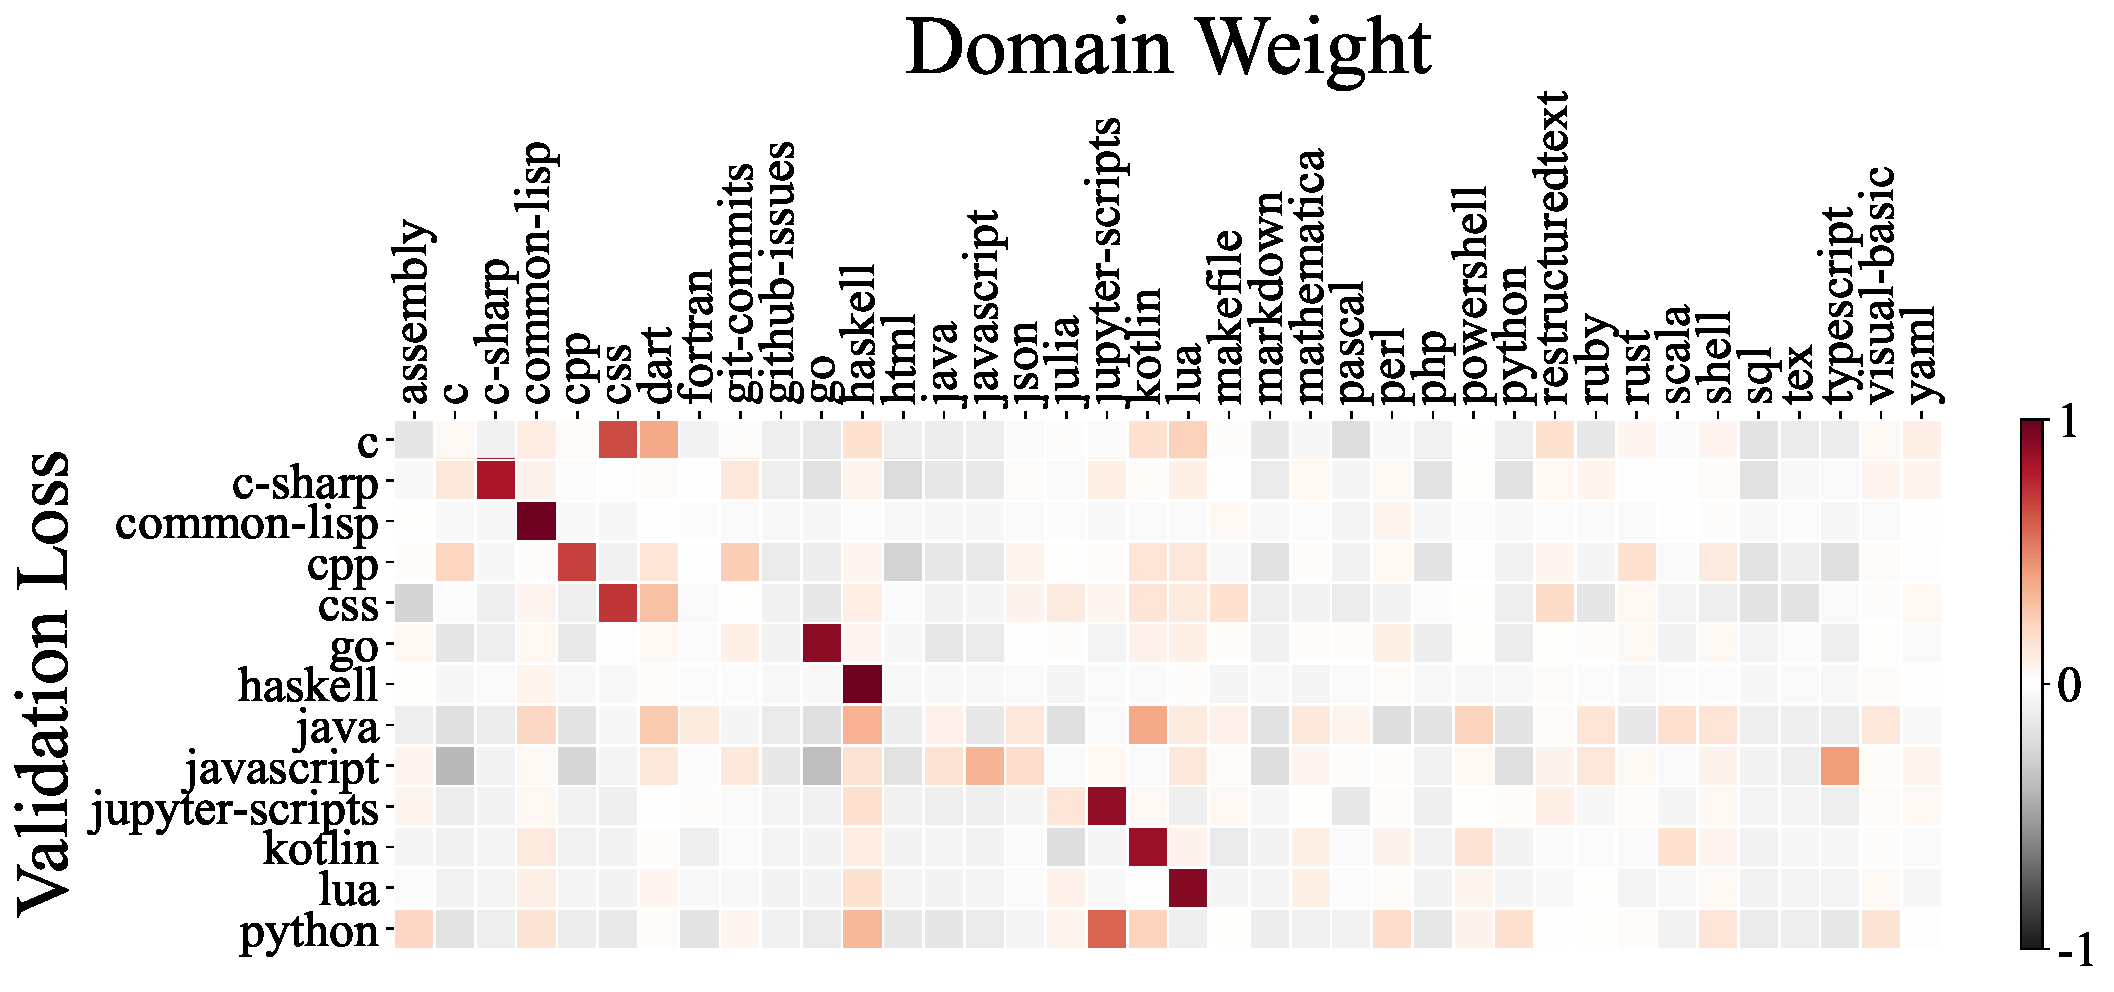
\includegraphics[height=.285\textwidth]{figures/1M_code_w.pdf}}
    \caption{The visualization of correlations between different target domain validation losses and training domain weights using the linear regression model. \textbf{Left} is on the Pile dataset, and \textbf{Right} is on the Stack dataset. A high correlation indicates that increasing the training domain weight has a positive impact on reducing the target domain validation loss.}
    \vspace{-1mm}
    \label{fig:domain_interaction}
\end{figure}

To understand the impact of different domains on each other, we visualize the coefficients ($\boldsymbol{\omega}$) of the linear regression model in Figure~\ref{fig:domain_interaction}. The visualization provides insights into how the various data domains contribute to the others, revealing complex interactions among them. We also display code correlation diagrams for each 1M code model trained on The Stack dataset~\citep{thestack2022paper}. Surprisingly, both the domain interaction visualization and the code correlation diagrams display complex relationships that are difficult for human experts to fully comprehend. For example, the PhilPapers domain in the Pile dataset appears to provide gains for all other domains under the linear regression modeling, which is a non-obvious finding that challenges intuitive human understanding. These visualizations highlight the inherent complexity in determining the optimal data mixture, underscoring the value of our automated \ourmethod approach in efficiently identifying high-performing mixtures, rather than relying solely on human intuition.


\subsection{Data mixture effects transcend scaling laws}

\begin{figure}[t]
    \centering
    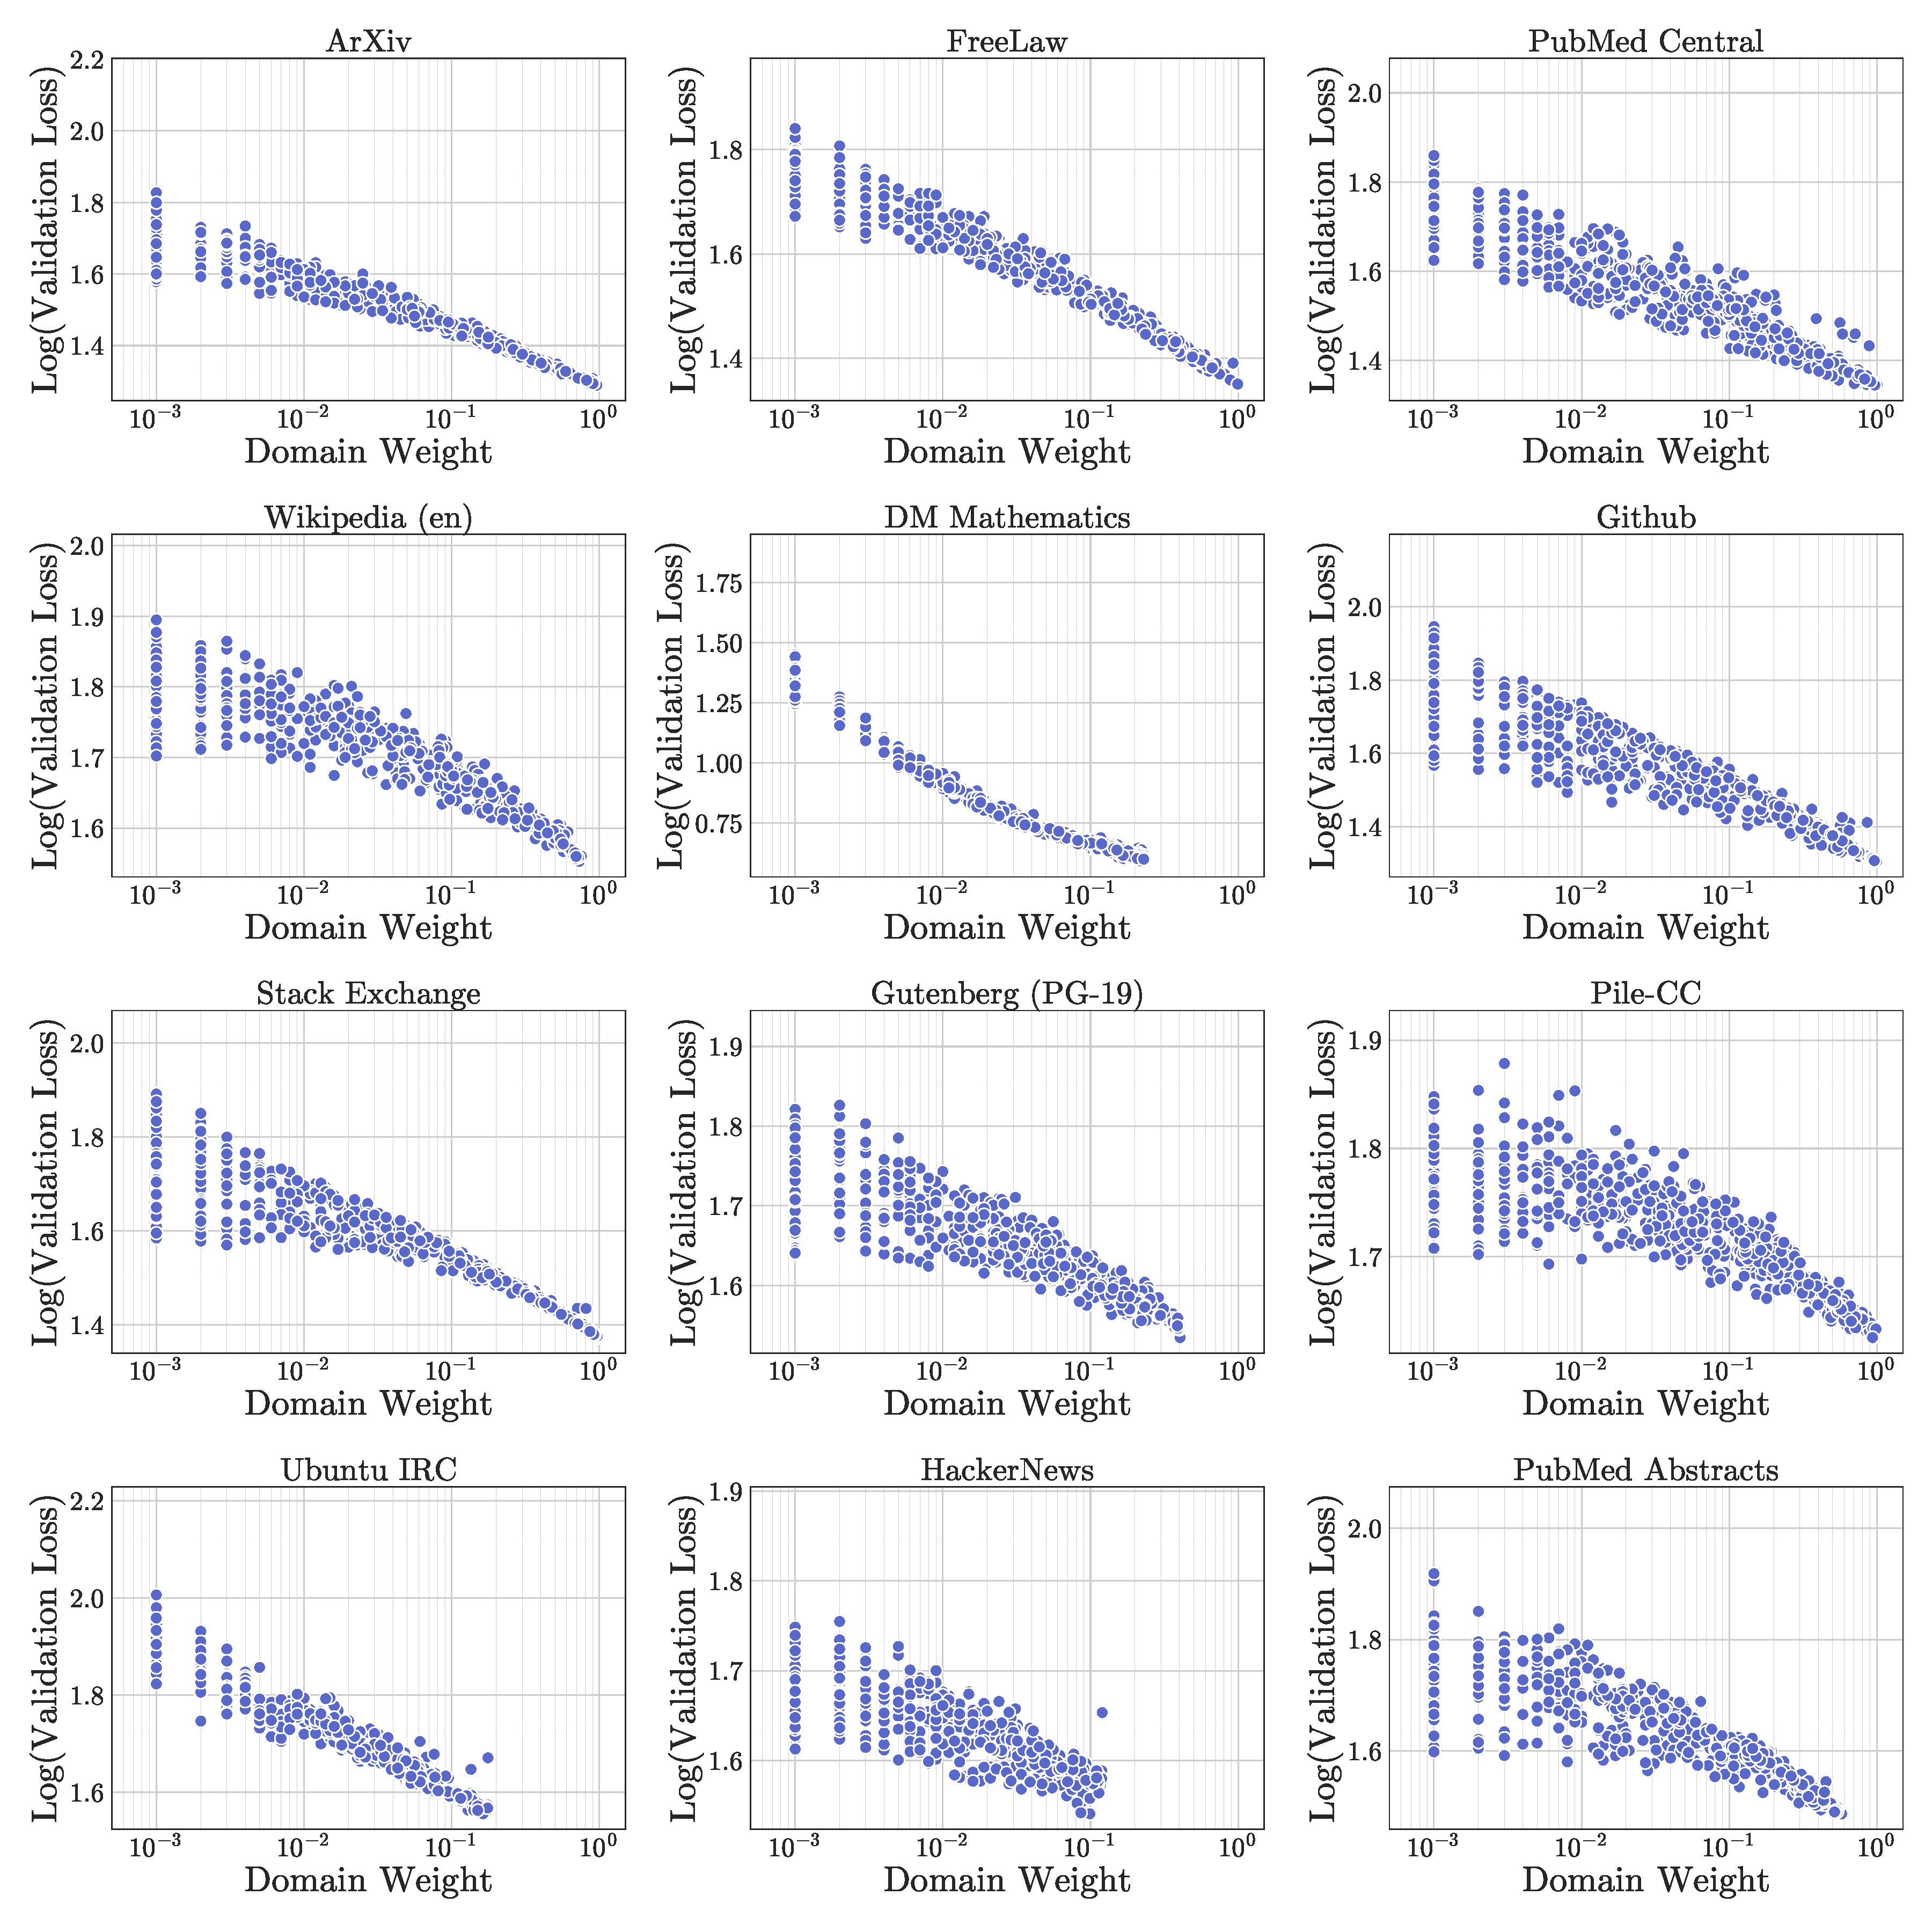
\includegraphics[width=0.8\textwidth]{figures/minimum_1024_log.pdf}
    \vspace{-3mm}
    \caption{The visualization of 1M training logs across various data mixtures. The x-axis represents the weight of each domain in the data mixture and the y-axis shows the log value of validation loss for that domain. As seen, predicting the validation loss solely based on the domain weight is challenging.\looseness=-1}
    \vspace{-2mm}
    \label{fig:log_loss_vs_weight}
\end{figure}

Recent research~\citep{ye2024datamixing,ge2024data} has demonstrated the feasibility of scaling laws for data mixture.
However, our findings in Section~\ref{sec:domain_interaction} suggest that the relationship between domain weights and validation loss is more complex than scaling laws might imply.
To visualize this complexity, we plotted all experimental points of our 1M training logs in Figure~\ref{fig:log_loss_vs_weight}.
If the scaling law of data mixture held true, we would expect to see a clear log-log linear relationship across all domains.
However, our results reveal a more nuanced picture.
For example, the DM Mathematics domain, possibly due to its distinct distribution compared to other domains, exhibits a near log-log linear relationship between loss and domain weight.
In contrast, for most domains like Pile-CC show more complex patterns, where predicting validation loss is non-trivial.
As shown, domain interactions appear to be intricate, making it challenging to predict the validation loss for a domain based solely on its weight in the mixture.
These findings suggest that while scaling laws provide valuable insights, they may not fully capture the intricacies of data mixture dynamics.
Our approach addresses the challenge by modeling the entire data mixture as input for the regression model, providing a more comprehensive framework for predicting the validation loss while simultaneously accounting for all domain weights.\looseness=-1



\subsection{Extend \ourmethod to 100 domains}

To demonstrate \ourmethod's scalability, we conducted preliminary experiments with 100 finer-grained domains. 
One key challenge lies in clustering web content into meaningful domain representations.
Intuitively, we define domains by base URLs from the FineWeb dataset~\citep{penedo2024fineweb}, chosen based on token availability. 
Example domains include \textit{articles.latimes.com}, \textit{blogs.wsj.com}, \textit{en.wikipedia.org}, \textit{everything2.com}, and \textit{techcrunch.com}. 

We train 1,000 small-scale models (1M parameters) across different data mixtures, use the training runs to fit a regression model and then predict the data mixture for models with 1M and 60M parameters. 
Rank correlation ($\rho$) and mean squared error (MSE) were evaluated for both linear and LightGBM regression models as shown in Table~\ref{tab:linear_vs_lightgbm_more_domains}.
The results demonstrate the effectiveness of \ourmethod when extending to 100 domains.


\begin{table}[t]
    \centering
    \small
    \caption{Performance Comparison on 100 Domains for 1M and 60M Models. This table compares the rank correlation ($\rho$, higher is better) and mean squared error (MSE, lower is better) for linear and LightGBM regression models. 
    We train 1,000 runs for 1M models, fit the regression model, and verify the rank correlation between the ranking predicted by the regression model and the ground-truth ranking of 64 unseen data mixtures on both 1M and 60M models.}
    \label{tab:linear_vs_lightgbm_more_domains}
    \vspace{1mm}
    \begin{tabular}{lccc}
        \toprule
        {Test On} & \multicolumn{2}{c}{\textit{1M}} & {\textit{60M}}  \\
        \cmidrule(lr){1-1} \cmidrule(lr){2-3}  \cmidrule(lr){4-4}
        \textbf{Method} & \textbf{$\rho$ ($\uparrow$)} & \textbf{MSE ($\downarrow$)} & \textbf{$\rho$ ($\uparrow$)} \\
        \midrule
        Linear & 90.33 & 0.12  & 88.64  \\
        {LightGBM} & {99.53} & {0.02} & {98.80} \\
        \bottomrule
    \end{tabular}
\end{table}

